% =====================================================================
\section{Theory}
\label{sec:theory}
% =====================================================================

\subsection{Physical model}
\label{sec:model}

% Written from the code as of 2026-11-02: nvision/spectra/nv_center.py and numba_kernels.py
% (signal), sim/gen/nv_center_generator.py and sim/presets.py (study grid), sim/combinations.py
% (SNR -> sigma). Code names: zero_field_freq = D, zeeman_shift = Delta_Z, hwhm = gamma,
% contrast_total = 2C (each Zeeman group carries half of it), noise_sigma = sigma.

The negatively charged N-V centre is described by five levels
\cite{manson2006,doherty2013nv} (Fig.~\ref{fig:levels}): the spin-triplet ground state $^3A_2$, split into
$|0\rangle_g$ and $|\pm1\rangle_g$ by the spin projection $m_s$ on the N-V axis; the spin-triplet excited state
$^3E$, with $|0\rangle_e$ and $|\pm1\rangle_e$; and a metastable spin singlet $|s\rangle$ that stands for the
singlet manifold. Green light drives the spin-conserving optical transitions $|m_s\rangle_g\to|m_s\rangle_e$, which
decay back by emitting red photoluminescence (PL). From $|\pm1\rangle_e$, however, the intersystem crossing to the
singlet is much faster than from $|0\rangle_e$, and the singlet decays preferentially to $|0\rangle_g$.
% The singlet -> |g,0> branching ratio is still debated: ~50-70 % (Robledo et al. 2011; Tetienne et al. 2012)
% vs ~90 % (Wirtitsch et al.), as summarised in arXiv:2511.19583. Not needed here: only the net pumping into
% m_s = 0 enters, through the rate Gamma_p below. Verify the primary sources before quoting a number.
Two
consequences follow. Under continuous illumination the spin is pumped into $m_s=0$; and a centre in $m_s=\pm1$
spends part of its optical cycles in the dark singlet, so it emits less PL than one in $m_s=0$. The spin state can
therefore be prepared and read out optically.
\begin{figure}[t]
\centering
\tbd{Level diagram: $^3A_2$ and $^3E$ triplets ($m_s=0,\pm1$), singlet $|s\rangle$; green pumping, red PL,
spin-selective intersystem crossing; microwave transitions at $D\pm\Delta_Z$.}
\caption{Five-level model of the N-V centre \cite{manson2006,doherty2013nv}. \tbd{Caption to follow the figure.}}
\label{fig:levels}
\end{figure}

With a static field $B_z$ along the N-V axis, the ground-state spin ($S=1$) Hamiltonian is, in units with
$h=1$ (energies in frequency units) \cite{doherty2013nv},
\begin{equation}
  H=D\,S_z^2+\gamma_e B_z S_z+A_\parallel S_zI_z ,
  \label{eq:hamiltonian}
\end{equation}
with $D\approx2.87$~GHz the zero-field splitting, $\gamma_e\approx28$~GHz/T the electron gyromagnetic ratio, and
$A_\parallel$ the axial hyperfine coupling to the nitrogen nuclear spin $I$ ($|A_\parallel|=2.15$~MHz for
$^{14}$N, $I=1$, and $3.03$~MHz for $^{15}$N, $I=1/2$ \cite{felton2009}). The strain splitting $E(S_x^2-S_y^2)$
is dropped, a small correction when $\gamma_e B_z\gg E$. The eigenstates are the product states
$|m_s,m_I\rangle$, and the magnetic-dipole transitions $m_s=0\to\pm1$, which conserve $m_I$, lie at
\begin{equation}
  f_\pm(m_I)=D\pm\left(\Delta_Z+A_\parallel m_I\right),\qquad \Delta_Z=\gamma_e B_z ,
  \label{eq:transitions}
\end{equation}
where $\Delta_Z$ is the Zeeman shift. Each electron transition therefore splits into $2I+1$ hyperfine lines
spaced by $|A_\parallel|$: a triplet for $^{14}$N and a doublet for $^{15}$N.

An ODMR measurement sets the microwave drive to a frequency $\nu$ and records the PL,
normalised to its off-resonant level. When $\nu$ meets $f_+$ or $f_-$, the drive transfers population from $m_s=0$ to
the darker $m_s=\pm1$ state and the PL dips. $D$ is treated as a known constant, so the position $f_+$ of the
upper line carries the field, $f_+-D=\Delta_Z$, and an uncertainty in $f_+$ is an uncertainty in $\Delta_Z$.

Near the excited-state level anticrossing the nitrogen nuclear spin is polarised into a single $m_I$, and each
transition shows a single line \cite{jacques2009}; its fixed offset $A_\parallel m_I$ is absorbed into $f_+$.
The same single line describes a line whose hyperfine structure is unresolved, $\Gamma\gg|A_\parallel|$.
The resolved triplet and doublet are treated at the end of this section. A drive near $f_+$ couples only $|0\rangle_g$ and $|+1\rangle_g$,
and the excited state and the singlet enter only through the rates at which the laser repolarises the spin and
destroys its coherence \cite{dreau2011}, so the spin is a driven two-level system $\{m_s=0,m_s=+1\}$. The
laser prepares it in $m_s=0$; a microwave drive of Rabi frequency $\Omega$ (Hz) at detuning $\Delta=\nu-f_+$ then
transfers it to $m_s=+1$ after a time $t$ with probability
\begin{equation}
  P(\Delta,t)=\frac{\Omega^2}{\Omega^2+\Delta^2}\,\sin^2\!\Big(\pi t\sqrt{\Omega^2+\Delta^2}\Big),
  \label{eq:rabi}
\end{equation}
and the PL dip is proportional to $P$. The line shape depends on how the drive is applied
(Fig.~\ref{fig:sequences}).
\begin{figure}[t]
\centering
\tbd{Sequence diagram: CW ODMR (laser and microwaves on together, PL read continuously) and pulsed ODMR
(laser pulse to polarise, microwave $\pi$-pulse of length $1/(2\Omega)$ with the laser off, laser pulse to read out).}
\caption{Laser and microwave sequences of CW and pulsed ODMR. \tbd{Caption to follow the figure.}}
\label{fig:sequences}
\end{figure}

\emph{CW ODMR.} Laser and microwaves are on together, and the spin is driven for a time $T$ much longer than one
Rabi period, $T\sqrt{\Omega^2+\Delta^2}\gg1$, while the laser keeps resetting the phase of the oscillation. Only the
time average of Eq.~\eqref{eq:rabi} is then seen, and since
$\frac1T\int_0^T\sin^2\!\big(\pi t\sqrt{\Omega^2+\Delta^2}\big)\,dt\to\tfrac12$ in this limit,
\begin{equation}
  \bar P(\Delta)=\frac12\,\frac{\Omega^2}{\Omega^2+\Delta^2},
  \label{eq:cw-lorentzian}
\end{equation}
a Lorentzian in $\Delta$ of half width $\Omega$. This is the microwave contribution to the width, power broadening:
the stronger the drive, the further off resonance it still flips the spin.

Eq.~\eqref{eq:cw-lorentzian} treats the drive alone. In CW ODMR the laser acts on the spin at the same time, in two
ways: each optical cycle pumps it back towards $m_s=0$, at a rate $\Gamma_p$, and destroys the phase between $m_s=0$
and $m_s=+1$, at a rate $\Gamma_c$. These are a longitudinal and a transverse relaxation rate, $1/T_1$ and $1/T_2$ of
the two-level system. The steady state of the Bloch equations with these rates and a drive of angular Rabi frequency
$\Omega_R=2\pi\Omega$ is \cite{dreau2011}
\begin{equation}
  P_{\rm ss}(\Delta)=\frac12\,\frac{\Omega_R^2\,\Gamma_c/\Gamma_p}{(2\pi\Delta)^2+\Gamma_c^2+\Omega_R^2\,\Gamma_c/\Gamma_p},
  \label{eq:bloch-ss}
\end{equation}
which reduces to Eq.~\eqref{eq:cw-lorentzian} when the two rates are equal. It is still a Lorentzian, now of half width
\begin{equation}
  \gamma=\frac{1}{2\pi}\sqrt{\Gamma_c^2+\Omega_R^2\,\frac{\Gamma_c}{\Gamma_p}} .
  \label{eq:linewidth}
\end{equation}
The two terms add in quadrature. The first is the optical broadening: the width that remains at vanishing microwave
power, set by how fast the laser destroys the spin's coherence. The second is the microwave power broadening of
Eq.~\eqref{eq:cw-lorentzian}, scaled by $\Gamma_c/\Gamma_p$. Both rates grow with the optical saturation parameter
$s$ as $\Gamma_{p,c}=\Gamma_{p,c}^\infty\,s/(1+s)$, so the line is set by the laser power at weak microwave drive and
by the microwave power at strong drive. The depth, the value of Eq.~\eqref{eq:bloch-ss} at $\Delta=0$, depends on both
powers as well \cite{dreau2011}.
% Dreau et al. (2011) Eq. 11 quotes the same width as Gamma_c^inf/(2 pi) sqrt((s/(1+s))^2 + Omega_R^2/(Gamma_p^inf
% Gamma_c^inf)) and calls it the FWHM; with Gamma_{p,c} = Gamma^inf s/(1+s) this is Eq. (linewidth) up to their
% factor-2 convention for the rates. Check before quoting numbers.
Whatever its origin, the line is one Lorentzian dip,
\begin{equation}
  S(\nu)=1-C\,\frac{\gamma^2}{\gamma^2+(\nu-f_+)^2},
  \label{eq:signal}
\end{equation}
with contrast $C$ (the depth of the dip), half width $\gamma$ of Eq.~\eqref{eq:linewidth} and full width at half
maximum $\Gamma=2\gamma$. Optical and microwave broadening are not modelled separately: they enter only through the single linewidth $\Gamma$,
which is inferred with the line. Eq.~\eqref{eq:signal} is the line used in Sec.~\ref{sec:fisher}.

\emph{Pulsed ODMR} is used to eliminate this power broadening \cite{dreau2011}. In CW ODMR, Eq.~\eqref{eq:linewidth},
the laser that reads the spin out also broadens the line through $\Gamma_c$, and narrowing it means lowering both powers and with them
the contrast and the PL. Pulsed ODMR separates the two in time: the laser first polarises the spin and is then
switched off while a single microwave $\pi$-pulse of duration $t_\pi=1/(2\Omega)$ is applied, after which a second
laser pulse reads the spin out (Fig.~\ref{fig:sequences}). The laser therefore no longer broadens the line, the
microwave width is set by the pulse length rather than by a steady drive power, and Eq.~\eqref{eq:rabi} is evaluated
at the one fixed time $t_\pi$ instead of being averaged. With $r=\sqrt{1+\Delta^2/\Omega^2}$,
\begin{equation}
  P_\pi(\Delta)=\frac{\sin^2(\pi r/2)}{r^2},
  \label{eq:pulsed}
\end{equation}
which is not a Lorentzian but a sinc$^2$-like line: for $|\Delta|\gg\Omega$, $r\approx|\Delta|/\Omega$ and
$P_\pi\approx\tfrac{\pi^2}{4}\,\mathrm{sinc}^2(\pi\Delta t_\pi)$, with $\mathrm{sinc}\,u=\sin u/u$: the
power spectrum of a rectangular pulse of length $t_\pi$. Its features follow from Eq.~\eqref{eq:pulsed}. On resonance
$r=1$ and the inversion is complete, $P_\pi=1$; the half width is $0.80\,\Omega$, so the line narrows as the pulse
gets longer, the Fourier limit $\propto1/t_\pi$. The line vanishes wherever $\sin(\pi r/2)=0$, i.e.\ $r=2,4,\dots$,
at $|\Delta|=\sqrt3\,\Omega,\sqrt{15}\,\Omega,\dots$: there the spin completes a whole number of full Rabi cycles
and returns to $m_s=0$. Between the zeros lie side lobes that decay as $1/r^2$; the first, near $r=3$ at
$|\Delta|\approx2.7\,\Omega$, is 12\% of the depth. Side lobes are a hazard for a search: a lobe is a dip where
there is no resonance.

$T_2^*$ sets how far this narrowing can go. The spin's transition frequency is not sharp but fluctuates from run
to run (mostly through the $^{13}$C nuclear-spin bath), a Gaussian spread of width
$\sigma_\delta=1/(\sqrt2\,\pi T_2^*)$, so the measured line is Eq.~\eqref{eq:pulsed} averaged over that spread,
\begin{equation}
  \bar P_\pi(\Delta)=\int P_\pi(\Delta-\delta)\,\frac{e^{-\delta^2/2\sigma_\delta^2}}{\sqrt{2\pi}\,\sigma_\delta}\,d\delta .
  \label{eq:pulsed-t2star}
\end{equation}
For $t_\pi\ll T_2^*$ the spread is small against $\Omega$ and the line is the sinc$^2$-like Eq.~\eqref{eq:pulsed}.
For $t_\pi\gtrsim T_2^*$ the Gaussian dominates: the zeros and side lobes are washed out, the line stops narrowing at
a width $\sim1/T_2^*$, and the depth falls because the pulse no longer inverts every frequency class
\cite{dreau2011}. The best pulsed line is therefore reached at $t_\pi\sim T_2^*$, a width set by the spin itself rather than by
the laser or microwave power. CW ODMR and its Lorentzian line are the main case of this work, and the information
analysis of Sec.~\ref{sec:fisher} is derived for it; pulsed ODMR is treated as well, with its own line shape,
Eq.~\eqref{eq:pulsed-t2star}, in place of Eq.~\eqref{eq:signal}. \tbd{Where pulsed goes (a Theory subsection for
the information of the pulsed line, and its own Results).}

% Code: NVCenterPulsedDriveModel (spectra/nv_center_drive.py) evaluates Eq. (rabi) with the Gaussian T2* average;
% NVCenterCWDriveModel broadens with MW power only, gamma = gamma_0 sqrt(1 + s_MW), gamma_0 = 150 kHz fixed, i.e.
% no optical term. The SNR x window study uses a fixed linewidth (no drive), consistent with one Gamma.

The spectrum is mirror symmetric about $D$, so the drive window is
placed above $D$ and holds the upper transition only. The tail of the lower one, at $D-\Delta_Z$, adds
$C\gamma^2/[\gamma^2+(\nu-D+\Delta_Z)^2]$ inside the window: at the line centre a fraction
$\gamma^2/(\gamma^2+4\Delta_Z^2)$ of $C$, i.e.\ 20\% at $\Delta_Z=\gamma$ and below 1\% for $\Delta_Z\gtrsim5\gamma$.
Equation~\eqref{eq:signal} assumes $\Delta_Z\gg\gamma$. Small Zeeman shifts, where the tails of the two lines
overlap, are a separate problem and outside the scope of this work.

$f_+$ is the parameter of interest. The width $\Gamma$ and the contrast $C$ are nuisance parameters: they are inferred
jointly with $f_+$ but only matter through their effect on it. The noise level $\sigma$ (below) is inferred as
well.

One shot is a PL reading at a fixed drive frequency. A shot that collects $N_{\rm ph}$ photons
on average has Poisson-distributed counts, so the normalised reading has a standard deviation of at least
$N_{\rm ph}^{-1/2}$ (to first order in $C$): the photon shot-noise limit, reached when technical noise (laser
intensity, microwave power, collection drift) is negligible. For $N_{\rm ph}\gg1$ the counts are close to Gaussian,
and the single-shot reading is
\begin{equation}
  y=S(\nu)+\epsilon,\qquad \epsilon\sim\mathcal N(0,\sigma^2),\qquad \sigma\ge N_{\rm ph}^{-1/2}.
  \label{eq:noise}
\end{equation}
A measurement is the mean of $k$ shots at the same $\nu$. Its noise is $\sigma/\sqrt k$, so its Fisher information,
Eq.~\eqref{eq:fisher}, grows linearly with $k$. At the shot-noise limit it grows with the total number of photons
$kN_{\rm ph}$ collected at that drive frequency, which no averaging scheme can beat. The signal-to-noise ratio of a
single shot depends on where it is taken: it is the drop in PL at $\nu$ over the noise,
\begin{equation}
  \mathrm{SNR}(\nu)=\frac{1-S(\nu)}{\sigma}=\frac{C}{\sigma}\,\frac{\gamma^2}{\gamma^2+(\nu-f_+)^2}.
  \label{eq:snr-local}
\end{equation}
It is largest on resonance, $\nu=f_+$, where
\begin{equation}
  \mathrm{SNR}\equiv\mathrm{SNR}(f_+)=C/\sigma ,
  \label{eq:snr}
\end{equation}
the single number by which a line is labelled. The information of a measurement, however, follows the local slope of
$S$ rather than its depth, Eq.~\eqref{eq:fisher}: it vanishes on resonance and peaks at $|\nu-f_+|=\gamma/\sqrt3$,
where the dip is $3/4$ deep, which gives Eq.~\eqref{eq:istar}. Equation~\eqref{eq:snr} also neglects the mirror
line: its tail raises the on-resonance depth to $C[1+\gamma^2/(\gamma^2+4\Delta_Z^2)]$, so $C/\sigma$ is the
$\Delta_Z\gg\gamma$ limit of the on-resonance SNR.
In the simulations each measurement is one Gaussian draw, i.e.\ $k=1$, and $\sigma$ is set from the SNR.
All SNR values in this paper follow Eq.~\eqref{eq:snr}.
% Code convention differs: the code's SNR label is contrast_total/sigma with contrast_total = 2C, so a run
% labelled SNR = x has C/sigma = x/2 here (and I* 4x smaller than the label suggests). Convert every
% simulated SNR by /2 before quoting it in figures, tables or text.

The prior knowledge of the experimentalist is an interval of width $W$ that holds the
resonance, $f_+\in[f_{\min},f_{\min}+W]$; $W$ is the prior support of $f_+$ that enters
Eq.~\eqref{eq:prior}, and the drive frequency is scanned over at least this interval. The ratio $W/\Gamma$, the
inverse of the fraction of the window the line occupies, sets how hard the search is.
\tbd{Code fix in progress: the particle filter's prior on $\Delta_Z$ becomes uniform over the range the truth is drawn
from (it is now an offset Gaussian plus 10\% uniform); the nuisance priors stay offset on purpose. Then state $W$ of
the simulations here: is it the drive window $W_{\rm d}$ or the $\Delta_Z$ range?}

The code also models a pseudo-Voigt line whose total width is the linear sum
$\Gamma=\Gamma_L+\Gamma_G$ of its Lorentzian and Gaussian parts (the study varies the Gaussian share at fixed
$\Gamma$), and the resolved hyperfine lines of Eq.~\eqref{eq:transitions}, a $^{14}$N triplet or a $^{15}$N doublet whose
lines share the same total contrast; the main text keeps the single Lorentzian of Eq.~\eqref{eq:signal}.
\tbd{Where the hyperfine-resolved runs are used, and how $f_+$ is defined for them (centre line or $m_I$-averaged).}

\subsection{Fisher information of a single measurement}
\label{sec:fisher}

From here on, the statistics are written in the common notation of Bayesian experimental design: the design
$x\equiv\nu$ is the drive frequency, $\theta\equiv f_+$ the parameter of interest, $\phi=(\Gamma,C)$ the nuisance
parameters, $y$ the outcome of a measurement, and $S(x;\theta,\phi)$ the line of Eq.~\eqref{eq:signal}.
One measurement at $x$, the mean of $k$ shots with single-shot noise $\sigma$, carries Fisher information about
$\theta$
\begin{equation}
  I(x)=\frac{k\,g(x)^2}{\sigma^2},\qquad g(x)=\frac{\partial S(x;\theta,\phi)}{\partial\theta}.
  \label{eq:fisher}
\end{equation}
For a Lorentzian dip of depth $C$ and full width $\Gamma$, $S=1-C\,\gamma^2/(\gamma^2+u^2)$ with
$\gamma=\Gamma/2$ and $u=x-\theta$, the slope is steepest at $|u|=\gamma/\sqrt3$, where
$|g^*|=9C/(4\sqrt3\,\Gamma)\approx1.30\,C/\Gamma$. The best possible information per measurement is therefore
\begin{equation}
  I^*=\max_x I(x)=\frac{27}{16}\,k\,\frac{\mathrm{SNR}^2}{\Gamma^2},\qquad \mathrm{SNR}=C/\sigma .
  \label{eq:istar}
\end{equation}
$I^*$ assumes the nuisance parameters (width, contrast) are known; with free nuisances it is an upper bound on the
usable information. The nuisances are inferred along with $\theta$ but are not the subject of this work.

\subsection{Prior information: the search window}
\label{sec:prior}

Information about $\theta$ is measured in inverse variance, $J=\sigma_\theta^{-2}$ (Hz$^{-2}$); independent
measurements add their $I(x)$ to it. The same currency measures what is known \emph{before} the first measurement.
If the experimentalist knows only that the resonance lies somewhere in a window of width $W$, the state of
knowledge is a uniform prior $p(\theta)=1/W$, whose variance is
\begin{equation}
  \sigma_0^2=\int_{-W/2}^{W/2}\frac{u^2}{W}\,du=\frac{W^2}{12},
  \qquad
  J_0\equiv\sigma_0^{-2}=\frac{12}{W^2}.
  \label{eq:prior}
\end{equation}
The search window is therefore a prior: it holds $J_0$ of information that no measurement had to pay for, and a
narrower window starts with more. (A uniform prior has no finite Fisher information at its edges, so the inverse
variance is used as the convention.) The unitless gain after the measurements is $\log_2(\sigma_0/\sigma)$ bits.
% \tbd: confirm J_0 = 12/W^2 (uniform window) rather than 1/sigma_prior^2 of a
% Gaussian prior; the simulated generators currently draw a Gaussian prior.

\subsection{Van Trees bound}
\label{sec:budget}

Because the prior carries information, the relevant bound is not the Cram\'er--Rao bound, which holds for
unbiased estimators and ignores $J_0$, but the van Trees inequality \cite{vantrees1968,gill1995}. It holds for
any estimator, averaged over the prior: measurements are independent given $\theta$, so their information adds
to the prior's,
\begin{equation}
  \sigma_\theta(N)\ \ge\ \Big(J_0+\sum_{n=1}^{N}I(x_n)\Big)^{-1/2}\ \ge\
  \sigma_B(N)=\Big(\frac{12}{W^2}+N I^*\Big)^{-1/2}.
  \label{eq:vantrees}
\end{equation}
The search, focus and refine regimes of a run are the limits of this bound and the crossover between them.

\paragraph{Prior limit (search).} For $\sum_n I(x_n)\ll J_0$, $\sigma\to\sigma_0=W/\sqrt{12}$: the knowledge is
still that of the window. The estimate leans on the prior and is biased towards its mean, which is why it may lie
below the unbiased Cram\'er--Rao bound.

\paragraph{Data limit (refine).} For $\sum_n I(x_n)\gg J_0$, the prior is washed out and the posterior mean
becomes asymptotically unbiased and efficient (Bernstein--von Mises \cite{vandervaart1998}): $\sigma_B$ tends to
the unbiased Cram\'er--Rao bound $(N I^*)^{-1/2}$ \cite{cramer1946}, a slope $-\tfrac12$ reached only by measuring
at the steepest slope.

\paragraph{Crossover (focus).} With $I^*$ at every step the crossover would come at
$N_c=J_0/I^*=\tfrac{64}{9}\,(\Gamma/W)^2/(k\,\mathrm{SNR}^2)$, far below one measurement for any realistic window
($N_c\approx2\times10^{-4}$ for $W=20\,\Gamma$ at $\mathrm{SNR}=10$). It comes much later because $I^*$ is reached
only once the dip has been found: a measurement on the baseline carries $I(x)\approx0$, so the sum in
Eq.~\eqref{eq:vantrees} stays near $J_0$ while the strategy searches. What such a measurement contributes instead
is \emph{elimination}: it shrinks the prior itself.

\paragraph{Elimination model.} Consider a sweep with spacing $\Delta$ (e.g.\ $\Delta=\Gamma/3$) at an SNR high
enough that one measurement inside the dip reveals it. After $n$ measurements without a dip, the posterior is
uniform on the part of the window not yet excluded, so
\begin{equation}
  \sigma(n)=\frac{W-n\Delta}{\sqrt{12}},\qquad n<n_d,
  \label{eq:elimination}
\end{equation}
where $n_d\le W/\Delta$ is the step that finds the dip (on average $W/(2\Delta)$ over a uniformly placed
resonance). In information terms $J(n)=12/(W-n\Delta)^2$: the gain per step is not constant but grows as the
remaining width shrinks. Detection localises the resonance to about one grid step, after which the measurements
add Fisher information:
\begin{equation}
  \sigma(n)=\Big(\frac{12}{\Delta^2}+(n-n_d)\,I^*\Big)^{-1/2},\qquad n\ge n_d .
  \label{eq:after-detection}
\end{equation}
Eqs.~\eqref{eq:elimination}--\eqref{eq:after-detection} reproduce both limits: $\sigma\to\sigma_0$ as $n\to0$ and
$\sigma\to(nI^*)^{-1/2}$ for $n\gg n_d$, the two limits of Eq.~\eqref{eq:vantrees}. For a wide window the
three regimes become visible (Fig.~\ref{fig:budget}): the prior limit is a plateau, since
Eq.~\eqref{eq:elimination} falls linearly and on a log--log axis looks flat until about half the window is excluded,
for a number of steps that grows with $W/\Delta$; the crossover is a cliff steeper than $-\tfrac12$, where
detection collapses $\sigma$ from about the window to about $\Delta$ (roughly $\log_2(W/\Delta)$ bits) and which
ends when the strategy can measure at the steepest slope, $\sigma\approx\varepsilon\approx0.075\,\Gamma$; the data
limit is the $-\tfrac12$ tail. A narrow window ($W\lesssim3.5\,\Gamma$, $\sigma_0\lesssim\Gamma$) has no plateau.
Search, focus and refine are therefore not separate mechanisms but the regimes of one bound.

The elimination model only illustrates the shape of the profile. At low SNR one measurement no longer reveals the
dip and $n_d$ grows, but Eq.~\eqref{eq:vantrees} holds at any SNR and needs no detection model; the runs are read
against it alone. The false-alarm test of Sec.~\ref{sec:locators} only steers where the strategy measures.

\begin{figure}[t]
\centering
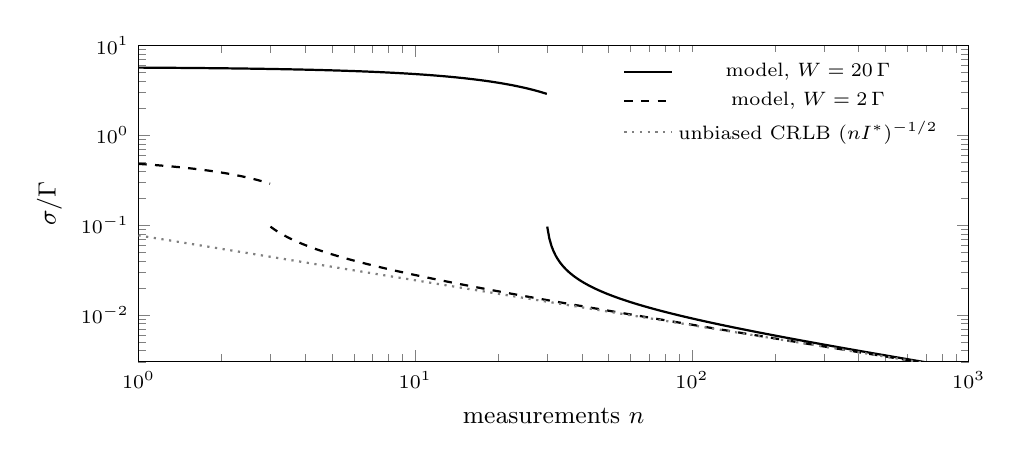
\begin{tikzpicture}
\begin{loglogaxis}[
  width=\linewidth, height=5.6cm,
  xlabel={measurements $n$}, ylabel={$\sigma/\Gamma$},
  xmin=1, xmax=1000, ymin=3e-3, ymax=10,
  legend style={font=\scriptsize, at={(0.98,0.98)}, anchor=north east, draw=none, fill=white},
  label style={font=\small}, tick label style={font=\scriptsize},
]
% Illustrative values: SNR = 10, k = 1, Delta = Gamma/3 -> I* = 168.75 / Gamma^2.
% Wide window W = 20 Gamma, dip found at n_d = 30 (half the 60-point grid).
\addplot[thick, domain=1:29.9, samples=60] {(20 - x/3)/sqrt(12)};
\addlegendentry{model, $W=20\,\Gamma$}
\addplot[thick, forget plot, domain=30:1000, samples=200] {1/sqrt(108 + 168.75*(x-30))};
% Narrow window W = 2 Gamma, n_d = 3 (half the 6-point grid).
\addplot[thick, dashed, domain=1:2.99, samples=20] {(2 - x/3)/sqrt(12)};
\addlegendentry{model, $W=2\,\Gamma$}
\addplot[thick, dashed, forget plot, domain=3:1000, samples=200] {1/sqrt(108 + 168.75*(x-3))};
\addplot[gray, dotted, thick, domain=1:1000, samples=100] {1/sqrt(168.75*x)};
\addlegendentry{unbiased CRLB $(nI^*)^{-1/2}$}
\end{loglogaxis}
\end{tikzpicture}
\caption{Elimination model, Eqs.~\eqref{eq:elimination}--\eqref{eq:after-detection}, at illustrative values
(SNR 10, $k=1$, $\Delta=\Gamma/3$, dip found halfway through the grid). The wide window shows a search plateau,
a detection cliff and the $-\tfrac12$ refine tail; the narrow window shows no plateau. Both start at the prior
limit $\sigma_0$ of the van Trees bound and tend to its data limit, the unbiased Cram\'er--Rao bound, at large $n$. \tbd{Schematic or drawn with the study's grid values?}}
\label{fig:budget}
\end{figure}

\subsection{Expected information gain and the bound}
\label{sec:eig}

The expected information gain of measuring at $x$ is the mutual information between the parameters and the
outcome, i.e.\ the expected Kullback--Leibler divergence from prior to posterior \cite{lindley1956}:
\begin{align}
  \mathrm{EIG}(x)&=\mathbb E_{y\mid x}\Big[D_{\rm KL}\big(p(\theta,\phi\mid y,x)\,\|\,p(\theta,\phi)\big)\Big]
  =I(\theta,\phi;y\mid x)\nonumber\\
  &=H[y\mid x]-\mathbb E_{\theta,\phi} H[y\mid\theta,\phi,x].
  \label{eq:eig-kl}
\end{align}
The noise is modelled as Gaussian with the same variance $\sigma^2/k$ at every drive frequency
(Sec.~\ref{sec:model}); this is an assumption of the model, not a limit, since otherwise every drive frequency would
need its own noise model. Hence, for a known $\sigma$, $H[y\mid\theta,\phi,x]=\tfrac12\ln(2\pi e\,\sigma^2/k)$; the
particle filter, which learns $\sigma$ (Sec.~\ref{sec:bayes}), uses its posterior mean. For a given variance the Gaussian
has the largest entropy \cite{cover2006}, so
$H[y\mid x]\le\tfrac12\ln 2\pi e\,(\sigma^2_{\rm pred}(x)+\sigma^2/k)$, with $\sigma^2_{\rm pred}(x)$ the variance of
$S(x;\theta,\phi)$ over the posterior. Hence
\begin{equation}
  \mathrm{EIG}(x)\le\tfrac12\ln\!\Big(1+\frac{k\,\sigma^2_{\rm pred}(x)}{\sigma^2}\Big),
  \label{eq:eig-var}
\end{equation}
which is what SBED (Sec.~\ref{sec:locators}) evaluates on its particles. Equality holds when the predictive distribution of
$S(x;\theta,\phi)$ is Gaussian.
% Code note: smc_marginal.py expected_information_gain uses the single-shot noise
% variance (no 1/k); the ranking is unchanged at fixed k.

\paragraph{When the variance is a good proxy: the local-linear regime.} The only remaining gap in
Eq.~\eqref{eq:eig-var} is the shape of the posterior. By the Bernstein--von Mises theorem, the Bayesian central limit
theorem \cite{vandervaart1998}, the posterior tends with growing data to a normal distribution centred near the
truth with variance $1/J_n$. A Gaussian's entropy depends on its variance alone,
$H[\theta]=\tfrac12\ln(2\pi e\,\sigma_\theta^2)$, so the expected KL divergence of one step reduces to a ratio of
variances, $\tfrac12\ln(\sigma_{\theta,n}^2/\sigma_{\theta,n+1}^2)$. Once the posterior is also narrow compared with
the line, $S$ is linear over it, the predictive distribution of $S(x;\theta,\phi)$ is Gaussian, Eq.~\eqref{eq:eig-var}
holds with equality, $\sigma^2_{\rm pred}(x)\approx g(x)^2\sigma_\theta^2$, and Eq.~\eqref{eq:eig-var} becomes
\begin{equation}
  \mathrm{EIG}(x)\approx\tfrac12\ln\big(1+I(x)\,\sigma_\theta^2\big)=\tfrac12\ln\frac{J_n+I(x)}{J_n}.
  \label{eq:eig-fisher}
\end{equation}
Greedy EIG then maximises $I(x)$, i.e.\ measures at the steepest slope, and the gains telescope:
$\sum_n\mathrm{EIG}_n=\tfrac12\ln(J_N/J_0)=\ln(\sigma_0/\sigma_N)$. The acquisition rule and the information budget
of Sec.~\ref{sec:budget} are the same quantity. The optimal strategy, which would measure every point at the
steepest slope of the true line, reaches the data limit of Eq.~\eqref{eq:vantrees}; greedy EIG approaches it once
the posterior is narrow compared with the line, while during the search it is only myopically optimal, which is
where the strategies of Sec.~\ref{sec:locators} differ.

\paragraph{When it is not: search.} Before the dip is found, the predictive distribution at $x$ is two-valued: with
probability $p$ (the posterior mass that would put a dip at $x$) the signal is $1-C$, otherwise 1. Then
$\sigma^2_{\rm pred}=p(1-p)C^2$, while the true mutual information is at most the binary entropy $H_b(p)$. The
variance form keeps growing with SNR where the true gain saturates, so it overvalues search candidates relative to
refine candidates; both peak at $p=\tfrac12$, so they rank search candidates alike.
\tbd{Mention computing the exact mixture entropy from the particles, or leave out?}

\subsection{Speedup over a frequency sweep}
\label{sec:speedup}

The same bound predicts the speedup over a conventional sweep. A sweep spreads its measurements uniformly over the
window, so its information per measurement is the window average of Eq.~\eqref{eq:fisher},
\begin{equation}
  \bar I=\frac{1}{W}\int I(x)\,dx=\frac{k}{\sigma^2W}\int g(x)^2\,dx=\frac{\pi}{4}\,
  \frac{k\,C^2}{\sigma^2\,\gamma\,W}
  \label{eq:sweep-info}
\end{equation}
for a Lorentzian ($\int(\partial_\theta L)^2d
u=\pi/4\gamma$), valid for $W\gg\Gamma$. The sweep therefore
accumulates information at the rate $\bar I$ from its first measurement, $\sigma\approx(J_0+N\bar I)^{-1/2}$, with no
plateau and no cliff, as observed by \citet{dushenko2020sbed}. An adaptive strategy pays the search cost $n_d$ first
and then gains $I^*$ per measurement. The number of measurements to reach a target $\tau$ is
\begin{equation}
  N_{\rm sweep}(\tau)=\frac{\tau^{-2}-J_0}{\bar I},\qquad
  N_{\rm ad}(\tau)=n_d+\frac{\tau^{-2}-12/\Delta^2}{I^*},
  \label{eq:n-to-target}
\end{equation}
and the speedup is $S(\tau)=N_{\rm sweep}/N_{\rm ad}$. For a precise target the refine terms dominate and
\begin{equation}
  S_\infty=\frac{I^*}{\bar I}=\frac{27}{16\pi}\,\frac{W}{\gamma}=\frac{27}{8\pi}\,\frac{W}{\Gamma}
  \approx1.07\,\frac{W}{\Gamma}.
  \label{eq:speedup}
\end{equation}
The speedup is set by the inverse occupancy $W/\Gamma$ of the window, which \citet{dushenko2020sbed} identified
qualitatively; Eq.~\eqref{eq:speedup} gives its prefactor. It is independent of the SNR, because both strategies
gain information $\propto\mathrm{SNR}^2$. For a loose target the search cost $n_d$ dominates $N_{\rm ad}$ and
$S(\tau)<S_\infty$, so the full dependence on window, linewidth, SNR (through $n_d$ at low SNR) and target is given
by Eq.~\eqref{eq:n-to-target}. A sweep cannot approach the van Trees bound at any $N$: its rate $\bar I$ is fixed by
the window, while the bound's data limit requires every measurement at the steepest slope.
\tbd{Check Eq.~\eqref{eq:speedup} against the speedup reported in Ref.~\cite{dushenko2020sbed} for their window
and line structure (a resolved triplet, not one Lorentzian).}

\subsection{Sensitivity and bandwidth}
\label{sec:sensitivity}

Sensitivity and bandwidth follow from the same budget once measurements are converted to time. Let one
measurement take $t_m=k\,t_s$ ($k$ shots of duration $t_s$), so that $T=N t_m$. With $D$ known, $f_+-D=\Delta_Z=\gamma_e B$ along
the N-V axis ($\gamma_e\approx28$~GHz/T), so $\sigma_B=\sigma_{f_+}/\gamma_e$.

\paragraph{Sensitivity (refine).} In the refine regime $\sigma_{f_+}=(N I^*)^{-1/2}$, so
$\sigma_{f_+}\sqrt T$ is a constant of the experiment:
\begin{equation}
  \eta=\frac{\sigma_{f_+}\sqrt T}{\gamma_e}=\frac{1}{\gamma_e}\sqrt{\frac{t_m}{I^*}}
  =\frac{4}{3\sqrt3}\,\frac{\Gamma\sqrt{t_s}}{\gamma_e\,\mathrm{SNR}_1},
  \label{eq:sensitivity}
\end{equation}
with $\mathrm{SNR}_1=C/\sigma$ the single-shot SNR. The prefactor $4/(3\sqrt3)$ is that of the standard CW-ODMR
sensitivity of a Lorentzian line \cite{dreau2011}: the familiar formula is the refine limit of the budget, reached
only by a strategy that measures at the steepest slope. A strategy whose refine measurements carry on average a
fraction $\bar\eta_F$ of $I^*$ reaches $\eta/\sqrt{\bar\eta_F}$.

\paragraph{Bandwidth (whole run).} A field reading is useful once the error reaches a target $\tau$; the time
needed, $T(\tau)$, sets the bandwidth $1/T(\tau)$. From the elimination model,
\begin{equation}
  T(\tau)=t_m\Big[n_d+\frac{\tau^{-2}-12/\Delta^2}{I^*}\Big],\qquad
  \eta_{\rm eff}(\tau)=\frac{\tau\sqrt{T(\tau)}}{\gamma_e}.
  \label{eq:bandwidth}
\end{equation}
For $\tau\to0$ the refine term dominates and $\eta_{\rm eff}\to\eta$ of Eq.~\eqref{eq:sensitivity}. For a loose
target the search term dominates: the bandwidth cannot exceed about $1/(n_d t_m)\sim\Delta/(W t_m)$, whatever the
SNR, and $\eta_{\rm eff}$ is worse than $\eta$. The window, i.e.\ the prior, therefore limits the bandwidth, while
the line shape and SNR limit the sensitivity. \tbd{Per-shot time is not yet in the simulated data, so results are
in measurements; take $t_s$ from the lab.}

